% ============================================================
% CHAPTER 4: SYSTEM DESIGN AND ARCHITECTURE
% ============================================================

\chapter{System Design and Architecture}

\section{Introduction to Solution Architecture}

System design bridges the gap between abstract requirements (Chapter 3) and concrete implementation (Chapter 5). This chapter presents the technical blueprint of the e-commerce platform through multiple architectural views, adhering to the **IEEE 1471-2000** standard for architecture description \cite{ieee1471}.

The design philosophy prioritizes:
\begin{itemize}
    \item \textbf{Separation of Concerns:} Clear boundaries between presentation, business logic, and data layers
    \item \textbf{Scalability:} Stateless architecture enabling horizontal scaling
    \item \textbf{Maintainability:} Modular design facilitating independent testing and updates
    \item \textbf{Security-by-Design:} Authentication/authorization baked into architecture, not retrofitted
\end{itemize}

The architecture is documented using multiple complementary models:
\begin{enumerate}
    \item **Logical Architecture:** High-level component view (client-server model)
    \item **Data Architecture:** Entity-Relationship Diagram (ERD) for MongoDB collections
    \item **API Architecture:** RESTful endpoint catalog with request/response schemas
    \item **Security Architecture:** Authentication flows and authorization mechanisms
    \item **Deployment Architecture:** Physical infrastructure and hosting topology
\end{enumerate}

\section{High-Level System Architecture}

\subsection{Client-Server Architectural Pattern}

The system follows the classical **Client-Server** model, a network architecture where:
\begin{itemize}
    \item **Clients** (web browsers) initiate requests for resources (HTML pages, product data, order submission)
    \item **Server** (Node.js Express application) processes requests, applies business logic, queries database, returns responses
    \item **Database** (MongoDB) persists application state (users, products, orders)
\end{itemize}

\begin{figure}[H]
\centering
\begin{tikzpicture}[
    node distance=2.5cm,
    box/.style={rectangle, draw, fill=blue!10, text width=4cm, text centered, rounded corners, minimum height=1.2cm, font=\small},
    db/.style={cylinder, draw, fill=green!10, text width=3cm, text centered, minimum height=1.5cm, shape border rotate=90, font=\small},
    arrow/.style={-latex, thick}
]
    % Clients
    \node [box] (browser) {Web Browser (Chrome, Firefox, Safari)};
    
    % Server Layer
    \node [box, below of=browser, yshift=-0.5cm] (express) {Express.js Application Server};
    \node [box, left of=express, xshift=-3cm] (auth) {Authentication Middleware (JWT)};
    \node [box, right of=express, xshift=3cm] (api) {REST API Endpoints};
    
    % Business Logic
    \node [box, below of=express, yshift=-0.5cm] (logic) {Business Logic Layer (Order Processing, Loyalty)};
    
    % Database
    \node [db, below of=logic, yshift=-1cm] (mongodb) {MongoDB Database (Users, Products, Orders, Carts)};
    
    % External Services
    \node [box, right of=mongodb, xshift=4cm, fill=orange!10] (gemini) {Google Gemini AI};
    \node [box, above of=gemini, fill=orange!10] (oauth) {Google OAuth 2.0};
    
    % Arrows
    \draw [arrow, <->] (browser) -- node[right, font=\tiny] {HTTP/HTTPS} (express);
    \draw [arrow] (express) -- (auth);
    \draw [arrow] (express) -- (api);
    \draw [arrow, <->] (express) -- (logic);
    \draw [arrow, <->] (logic) -- (mongodb);
    \draw [arrow, <->] (logic) -- node[above, font=\tiny] {API Call} (gemini);
    \draw [arrow, <->] (express) -- node[above, font=\tiny, sloped] {OAuth Flow} (oauth);
    
\end{tikzpicture}
\caption{High-Level Client-Server Architecture}
\label{fig:client_server}
\end{figure}

\subsection{Modular Monolith Architecture}

Within the server application, a **Modular Monolith** architecture organizes code into logical modules with well-defined responsibilities:

\begin{table}[H]
\centering
\caption{System Modules and Responsibilities}
\label{tab:modules}
\begin{tabular}{@{}p{0.25\linewidth}p{0.35\linewidth}p{0.30\linewidth}@{}}
\toprule
\textbf{Module} & \textbf{Responsibility} & \textbf{Key Files} \\
\midrule
\textbf{Authentication} & User registration, login, JWT issuance, Google OAuth integration & \texttt{server.js} lines 236-266, 180-228 \\
\textbf{Product Catalog} & Product search, filtering, sorting, pagination & \texttt{server.js} lines 276-283, \texttt{model/Product.js} \\
\textbf{Shopping Cart} & Add/remove items, cart synchronization (LocalStorage ↔ DB) & \texttt{server.js} lines 286-316, \texttt{store.html} \\
\textbf{Order Processing} & Checkout, stock validation, voucher application, order creation & \texttt{server.js} lines 348-430, \texttt{checkout.html} \\
\textbf{Loyalty System} & Points calculation, rank upgrades, voucher redemption & \texttt{server.js} lines 318-345, 416-426 \\
\textbf{Admin Dashboard} & Inventory management, order status updates, analytics & \texttt{admin/dashboard.html}, \texttt{server.js} lines 450-505 \\
\textbf{AI Chatbot} & Natural language query processing, product recommendations & \texttt{server.js} lines 509-754 \\
\bottomrule
\end{tabular}
\end{table}

\textbf{Design Rationale:} Modules are **logically separated** but **physically collocated** in a single codebase (\texttt{server.js}). This approach:
\begin{itemize}
    \item Maintains simplicity for academic scope (single deployment unit)
    \item Preserves module boundaries for future microservices extraction
    \item Avoids distributed systems complexity (inter-service communication, eventual consistency)
\end{itemize}

\section{Database Design}

\subsection{MongoDB Schema Architecture}

Unlike traditional relational databases with rigid schemas enforced via DDL (Data Definition Language), MongoDB employs **flexible schemas** defined programmatically via Mongoose ODM. However, this flexibility does not imply chaos; the system enforces schema constraints through Mongoose schema definitions.

\subsection{Entity-Relationship Model}

The following diagram illustrates logical relationships between MongoDB collections (analogous to ER diagrams for SQL databases):

\begin{figure}[H]
\centering
\begin{tikzpicture}[
    entity/.style={rectangle, draw, fill=blue!10, text width=3cm, text centered, minimum height=1cm, font=\small\bfseries},
    attribute/.style={ellipse, draw, fill=yellow!10, text width=2cm, text centered, font=\tiny},
    relationship/.style={diamond, draw, fill=green!10, text width=2cm, text centered, aspect=2, font=\tiny},
    line/.style={draw, -latex}
]
    % Entities
    \node [entity] (user) at (0, 0) {User};
    \node [entity] (product) at (6, 0) {Product};
    \node [entity] (cart) at (0, -4) {Cart};
    \node [entity] (order) at (6, -4) {Order};
    \node [entity] (voucher) at (3, -6.5) {Voucher};
    
    % Relationships
    \node [relationship] (has_cart) at (0, -2) {has};
    \node [relationship] (places) at (3, -2) {places};
    \node [relationship] (contains_p) at (6, -2) {contains};
    \node [relationship] (redeems) at (1.5, -5.5) {redeems};
    
    % Lines
    \draw [line] (user) -- node[left, font=\tiny] {1} (has_cart);
    \draw [line] (has_cart) -- node[left, font=\tiny] {1} (cart);
    
    \draw [line] (user) -- node[above, font=\tiny] {1} (places);
    \draw [line] (places) -- node[above, font=\tiny] {N} (order);
    
    \draw [line] (product) -- node[right, font=\tiny] {N} (contains_p);
    \draw [line] (contains_p) -- node[right, font=\tiny] {M} (order);
    
    \draw [line] (user) -- (redeems);
    \draw [line] (redeems) -- (voucher);
    
    % Attributes (sample)
    \node [attribute, above of=user, yshift=-0.8cm] {email};
    \node [attribute, left of=user, xshift=0.8cm] {password};
    \node [attribute, right of=product, xshift=-0.8cm] {name};
    \node [attribute, above of=product, yshift=-0.8cm] {price};
    
\end{tikzpicture}
\caption{Entity-Relationship Diagram (MongoDB Collections)}
\label{fig:erd}
\end{figure}

\subsection{Collection Schemas}

\subsubsection{Users Collection}

\begin{lstlisting}[language=JavaScript, caption=User Schema (server.js:91-101)]
const userSchema = new mongoose.Schema({
    email: { 
        type: String, 
        required: true, 
        unique: true,      // Enforces MongoDB unique index
        lowercase: true    // Normalizes email to lowercase
    },
    password: { 
        type: String, 
        required: true     // Bcrypt hash, never plaintext
    },
    role: { 
        type: String, 
        default: 'user'    // RBAC: 'user' or 'admin'
    },
    rank: { 
        type: String, 
        enum: ['Silver', 'Gold', 'VIP'],  // Loyalty tier
        default: 'Silver' 
    },
    points: { type: Number, default: 0 },
    totalSpending: { type: Number, default: 0 },
    
    // EMBEDDED SUBDOCUMENT: User's redeemed vouchers
    myVouchers: [{
        code: String,
        discountAmount: Number,
        isUsed: { type: Boolean, default: false },
        redeemedAt: { type: Date, default: Date.now }
    }]
}, { timestamps: true }); // Auto-creates createdAt, updatedAt
\end{lstlisting}

\textbf{Design Decisions:}
\begin{itemize}
    \item **Embedded Vouchers:** The \texttt{myVouchers} array is embedded within User documents rather than referenced to a separate collection. This **denormalization** trades storage space for query performance—fetching user profile retrieves all voucher data in a single read.
    \item **Unique Email Index:** The \texttt{unique: true} constraint creates a MongoDB unique index on the \texttt{email} field, preventing duplicate registrations at the database level (atomic operation, race-condition-safe).
\end{itemize}

\subsubsection{Products Collection}

\begin{lstlisting}[language=JavaScript, caption=Product Schema (model/Product.js)]
const productSchema = new mongoose.Schema({
    name: { type: String, required: true },
    price: { type: Number, required: true },
    short_description: { type: String },
    spec: { type: String },
    image_url: { type: String },
    category: { 
        type: String,
        enum: ['Mac', 'iPhone', 'iPad', 'Watch', 'HeadPhone'] 
    },
    stock: { type: Number, default: 100 }
}, { timestamps: true });

// COMPOUND TEXT INDEX for full-text search
productSchema.index({
    name: 'text',
    short_description: 'text',
    spec: 'text'
});
\end{lstlisting}

\textbf{Text Index Strategy:}
The compound text index enables efficient full-text search queries. When a user searches for "macbook pro m3", MongoDB's text indexing algorithm:
\begin{enumerate}
    \item Tokenizes the query into terms: ["macbook", "pro", "m3"]
    \item Searches the inverted index for documents containing these terms
    \item Ranks results by relevance score (TF-IDF algorithm)
\end{enumerate}

Without this index, MongoDB would perform a \texttt{\$regex} scan on every document—\textbf{O(n)} complexity, unacceptable for large catalogs.

\subsubsection{Orders Collection}

\begin{lstlisting}[language=JavaScript, caption=Order Schema with Embedded Items (server.js:134-148)]
const orderSchema = new mongoose.Schema({
    userId: { 
        type: mongoose.Schema.Types.ObjectId, 
        ref: 'User'  // Reference to User collection (JOIN analogy)
    },
    recipientName: { type: String, required: true },
    recipientPhone: { type: String, required: true },
    recipientAddress: { type: String, required: true },
    recipientNotes: String,
    paymentMethod: { type: String, required: true },
    
    // EMBEDDED ORDER ITEMS (denormalized for performance)
    items: [{ 
        name: String,
        price: String,  // Snapshot of price at order time (string with formatting)
        qty: Number,
        image: String
    }],
    
    totalAmountString: String,     // Display string: "29,990,000 ₫"
    totalAmountNumeric: Number,    // Raw number for calculations
    finalAmount: Number,           // After discounts
    appliedVoucher: { type: String, default: null },
    status: { 
        type: String, 
        enum: ['Pending', 'Shipped', 'Completed', 'Cancelled'],
        default: 'Pending' 
    }
}, { timestamps: true });
\end{lstlisting}

\textbf{Normalization vs. Denormalization Trade-Off:}

\begin{table}[H]
\centering
\caption{Order Items Storage Strategy Analysis}
\label{tab:order_items_tradeoff}
\small
\begin{tabular}{@{}p{0.22\linewidth}p{0.35\linewidth}p{0.35\linewidth}@{}}
\toprule
\textbf{Approach} & \textbf{Normalized (Separate OrderItems Collection)} & \textbf{Denormalized (Embedded Array)} \\
\midrule
\textbf{Storage Efficiency} & Higher. Product names stored once. & Lower. Duplicated across orders. \\
\textbf{Query Performance} & Slower. Requires \texttt{\$lookup} (JOIN). & Faster. Single document read. \\
\textbf{Historical Accuracy} & Risk of price changes affecting past orders. & Price snapshot preserved. \\
\textbf{Implementation} & Complex. Transactional writes required. & Simple. Atomic document insert. \\
\textbf{Selected For} & Analytics, reporting. & E-commerce order history (\checkmark). \\
\bottomrule
\end{tabular}
\end{table}

\textbf{Decision:} Denormalized embedded approach selected for:
\begin{itemize}
    \item **Auditability:** Order records must preserve exact item prices at purchase time (regulatory requirement for financial auditing).
    \item **Performance:** Displaying order history (common operation) requires no JOINs.
\end{itemize}

\subsubsection{Carts Collection}

\begin{lstlisting}[language=JavaScript, caption=Cart Schema (server.js:125-132)]
const cartSchema = new mongoose.Schema({
    userId: { 
        type: mongoose.Schema.Types.ObjectId, 
        ref: 'User', 
        required: true, 
        unique: true  // One cart per user
    },
    items: [{
        productId: { type: mongoose.Schema.Types.ObjectId, ref: 'Product' },
        name: String,
        quantity: { type: Number, default: 1 },
        price: Number,
        image_url: String
    }]
}, { timestamps: true });
\end{lstlisting}

\textbf{Cart-User Relationship:} The \texttt{unique: true} constraint on \texttt{userId} enforces a **one-to-one** relationship—each user has exactly one cart. This prevents orphaned carts and simplifies cart retrieval logic.

\section{API Design and Specification}

The system exposes a **RESTful API** adhering to HTTP/1.1 semantics and JSON data interchange format. All endpoints follow the pattern: \texttt{/api/<resource>/<action>}.

\subsection{Authentication Endpoints}

\begin{table}[H]
\centering
\caption{Authentication API Endpoints}
\label{tab:api_auth}
\small
\begin{tabular}{@{}p{0.15\linewidth}p{0.30\linewidth}p{0.45\linewidth}@{}}
\toprule
\textbf{Method} & \textbf{Endpoint} & \textbf{Description \& Request/Response} \\
\midrule
\texttt{POST} & \texttt{/api/register} & 
\textbf{Request:} \texttt{\{"email": "user@example.com", "password": "SecurePass123"\}} \\
& & \textbf{Response (201):} \texttt{\{"message": "Registration successful"\}} \\
& & \textbf{Error (400):} Email already exists \\
\midrule
\texttt{POST} & \texttt{/api/login} & 
\textbf{Request:} \texttt{\{"email": "...", "password": "..."\}} \\
& & \textbf{Response (200):} \texttt{\{"\_id": "...", "email": "...", "role": "user", "accessToken": "eyJhbG..."\}} \\
& & \textbf{Error (401):} Invalid credentials \\
\midrule
\texttt{GET} & \texttt{/api/users/profile} & 
\textbf{Headers:} \texttt{token: Bearer \{JWT\}} \\
& & \textbf{Response (200):} \texttt{\{"user": \{...\}, "orders": [...]\}} \\
& & \textbf{Error (401):} Missing/invalid token \\
\bottomrule
\end{tabular}
\end{table}

\subsection{Product Catalog Endpoints}

\begin{table}[H]
\centering
\caption{Product API Endpoints}
\label{tab:api_products}
\small
\begin{tabular}{@{}p{0.15\linewidth}p{0.30\linewidth}p{0.45\linewidth}@{}}
\toprule
\textbf{Method} & \textbf{Endpoint} & \textbf{Description \& Parameters} \\
\midrule
\texttt{GET} & \texttt{/api/products/search} & 
\textbf{Query Params:} \texttt{q} (search term), \texttt{limit} (max results) \\
& & \textbf{Example:} \texttt{/api/products/search?q=iphone\&limit=20} \\
& & \textbf{Response:} \texttt{\{"products": [\{name, price, image\_url, category, stock\}]\}} \\
& & \textbf{Search Logic:} MongoDB \texttt{\$regex} on \texttt{name} field (case-insensitive) \\
\bottomrule
\end{tabular}
\end{table}

\subsection{Shopping Cart Endpoints}

\begin{table}[H]
\centering
\caption{Cart API Endpoints}
\label{tab:api_cart}
\small
\begin{tabular}{@{}p{0.15\linewidth}p{0.30\linewidth}p{0.45\linewidth}@{}}
\toprule
\textbf{Method} & \textbf{Endpoint} & \textbf{Description} \\
\midrule
\texttt{GET} & \texttt{/api/cart} & 
\textbf{Auth:} Required (JWT) \\
& & \textbf{Response:} Returns user's cart with items array \\
\midrule
\texttt{POST} & \texttt{/api/cart/add} & 
\textbf{Request:} \texttt{\{productId, quantity, name, price, image\_url\}} \\
& & \textbf{Logic:} If item exists, increment quantity; else push new item \\
& & \textbf{Response:} Updated cart document \\
\midrule
\texttt{DELETE} & \texttt{/api/cart/item/:productId} & 
\textbf{Param:} MongoDB ObjectId of product \\
& & \textbf{Logic:} Filters out item from \texttt{items} array, saves cart \\
\bottomrule
\end{tabular}
\end{table}

\subsection{Order Processing Endpoints}

\begin{table}[H]
\centering
\caption{Order API Endpoints}
\label{tab:api_orders}
\small
\begin{tabular}{@{}p{0.15\linewidth}p{0.35\linewidth}p{0.40\linewidth}@{}}
\toprule
\textbf{Method} & \textbf{Endpoint} & \textbf{Description} \\
\midrule
\texttt{POST} & \texttt{/api/orders} & 
\textbf{Auth:} Optional (supports guest checkout via token header) \\
& & \textbf{Request Body:} \\
& & \texttt{\{recipientName, recipientPhone, recipientAddress, recipientNotes, paymentMethod, items: [\{name, qty, ...\}], appliedVoucher\}} \\
& & \textbf{Business Logic:} \\
& & 1. Validate stock availability \\
& & 2. Calculate total (\texttt{price × qty}) \\
& & 3. Apply voucher discount if valid \\
& & 4. Deduct stock atomically \\
& & 5. Create Order document \\
& & 6. Clear user cart \\
& & 7. Award loyalty points \\
& & 8. Check rank upgrade \\
& & \textbf{Response (201):} \texttt{\{message: "Order successful", order: \{\_id, ...\}\}} \\
\midrule
\texttt{GET} & \texttt{/api/orders/:id} & 
\textbf{Auth:} None (public order tracking) \\
& & \textbf{Param:} MongoDB ObjectId \\
& & \textbf{Response:} Full order details (status, items, total) \\
& & \textbf{Error (404):} Order not found \\
\bottomrule
\end{tabular}
\end{table}

\subsection{Admin Endpoints}

\begin{table}[H]
\centering
\caption{Admin API Endpoints (Protected)}
\label{tab:api_admin}
\small
\begin{tabular}{@{}p{0.15\linewidth}p{0.40\linewidth}p{0.35\linewidth}@{}}
\toprule
\textbf{Method} & \textbf{Endpoint} & \textbf{Description} \\
\midrule
\texttt{GET} & \texttt{/api/admin/products} & 
\textbf{Auth:} Admin only (\texttt{verifyAdmin} middleware) \\
& & Returns all products with stock levels \\
\midrule
\texttt{PUT} & \texttt{/api/admin/products/:id/stock} & 
\textbf{Request:} \texttt{\{newStock: 50\}} \\
& & Updates product inventory \\
\midrule
\texttt{GET} & \texttt{/api/admin/orders} & 
Returns all orders with user email (populated) \\
\midrule
\texttt{PUT} & \texttt{/api/admin/orders/:id/status} & 
\textbf{Request:} \texttt{\{status: "Completed"\}} \\
& & Updates order lifecycle state \\
\midrule
\texttt{POST} & \texttt{/api/admin/vouchers} & 
\textbf{Request:} \texttt{\{code, discountAmount, pointsRequired, quantity\}} \\
& & Creates new loyalty voucher \\
\bottomrule
\end{tabular}
\end{table}

\section{Component Design}

\subsection{Middleware Architecture}

Express.js operates on a **middleware pipeline**—a chain of functions processing HTTP requests sequentially. Each middleware can:
\begin{itemize}
    \item Modify request/response objects
    \item Execute code (logging, authentication)
    \item Call \texttt{next()} to pass control to the next middleware
    \item Terminate the request-response cycle (send response)
\end{itemize}

\begin{figure}[H]
\centering
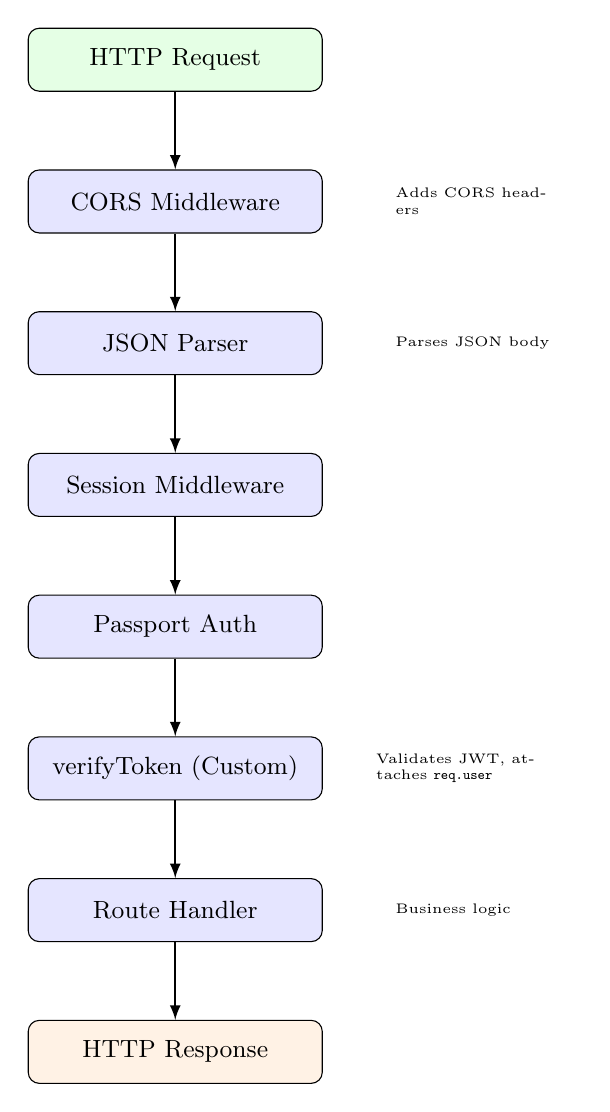
\begin{tikzpicture}[
    node distance=1.8cm,
    box/.style={rectangle, draw, fill=blue!10, text width=3.5cm, text centered, rounded corners, minimum height=0.8cm, font=\small},
    arrow/.style={-latex, thick}
]
    \node [box, fill=green!10] (request) {HTTP Request};
    \node [box, below of=request] (cors) {CORS Middleware};
    \node [box, below of=cors] (json) {JSON Parser};
    \node [box, below of=json] (session) {Session Middleware};
    \node [box, below of=session] (passport) {Passport Auth};
    \node [box, below of=passport] (verify) {verifyToken (Custom)};
    \node [box, below of=verify] (route) {Route Handler};
    \node [box, below of=route, fill=orange!10] (response) {HTTP Response};
    
    \draw [arrow] (request) -- (cors);
    \draw [arrow] (cors) -- (json);
    \draw [arrow] (json) -- (session);
    \draw [arrow] (session) -- (passport);
    \draw [arrow] (passport) -- (verify);
    \draw [arrow] (verify) -- (route);
    \draw [arrow] (route) -- (response);
    
    % Side annotations
    \node[right of=cors, xshift=2cm, font=\tiny, text width=2cm, align=left] {Adds CORS headers};
    \node[right of=json, xshift=2cm, font=\tiny, text width=2cm, align=left] {Parses JSON body};
    \node[right of=verify, xshift=2cm, font=\tiny, text width=2.5cm, align=left] {Validates JWT, attaches \texttt{req.user}};
    \node[right of=route, xshift=2cm, font=\tiny, text width=2cm, align=left] {Business logic};
    
\end{tikzpicture}
\caption{Express.js Middleware Pipeline}
\label{fig:middleware_pipeline}
\end{figure}

\section{Security Architecture}

\subsection{Authentication Flow: JWT-Based}

\begin{figure}[H]
\centering
\begin{tikzpicture}[
    node distance=1.5cm,
    actor/.style={rectangle, draw, fill=yellow!10, text width=2.5cm, text centered, minimum height=0.8cm, font=\small},
    server/.style={rectangle, draw, fill=blue!10, text width=2.5cm, text centered, minimum height=0.8cm, font=\small},
    db/.style={cylinder, draw, fill=green!10, text width=2cm, text centered, minimum height=1cm, shape border rotate=90, font=\small},
    arrow/.style={-latex, thick}
]
    \node [actor] (client) {Client (Browser)};
    \node [server, right of=client, xshift=4cm] (express) {Express Server};
    \node [db, right of=express, xshift=4cm] (mongo) {MongoDB};
    
    % Login Flow
    \draw [arrow] (client) -- ++(3.5,0) node[midway, above, font=\tiny] {POST /api/login} node[midway, below, font=\tiny] {\{email, password\}};
    \draw [arrow] (express) -- ++(3.5,0) node[midway, above, font=\tiny] {Find user by email};
    \draw [arrow] (mongo) -- ++(-3.5,0) node[midway, below, font=\tiny] {User document};
    \draw [arrow] (express) -- ++(-3.5,0) node[midway, below, font=\tiny, text width=2cm, align=center] {JWT token + user data};
    
    % Subsequent Requests
    \draw [arrow, dashed] ($(client) + (0,-1.5)$) -- ++(3.5,0) node[midway, above, font=\tiny] {GET /api/cart} node[midway, below, font=\tiny] {Header: token: Bearer \{JWT\}};
    \draw [arrow, dashed] ($(express) + (0,-1.5)$) -- ++(0,-0.5) node[right, font=\tiny, text width=2.5cm, align=left] {Verify JWT signature, Extract userId};
    \draw [arrow, dashed] ($(express) + (0,-2)$) -- ++(3.5,0) node[midway, above, font=\tiny] {Query cart by userId};
    
\end{tikzpicture}
\caption{JWT Authentication Sequence Diagram}
\label{fig:jwt_flow}
\end{figure}

\textbf{Security Mechanisms:}
\begin{enumerate}
    \item **Password Hashing:** Bcrypt with 10 salt rounds (computational cost = 2\textsuperscript{10} = 1024 iterations). This delay (≈100ms per hash) thwarts brute-force attacks.
    
    \item **JWT Payload:** Tokens contain minimal data (\texttt{userId}, \texttt{role}, \texttt{exp}), not sensitive fields (password hash, credit card). Payload is base64-encoded, **not encrypted**—confidentiality relies on HTTPS.
    
    \item **Token Expiration:** 3-day validity balances security (shorter = better) vs. UX (frequent re-login annoyance). Production systems should use 15-minute access tokens + refresh token rotation.
\end{enumerate}

\subsection{OAuth 2.0 Integration Flow}

\begin{figure}[H]
\centering
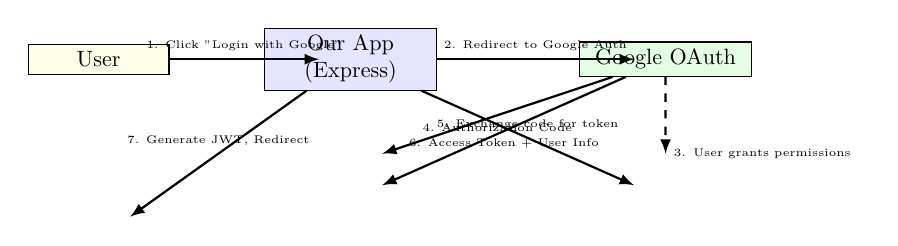
\begin{tikzpicture}[scale=0.8, every node/.style={scale=0.8}]
    \node[draw, rectangle, fill=yellow!10, text width=2cm, text centered] (user) at (0,0) {User};
    \node[draw, rectangle, fill=blue!10, text width=2.5cm, text centered] (app) at (4,0) {Our App (Express)};
    \node[draw, rectangle, fill=green!10, text width=2.5cm, text centered] (google) at (9,0) {Google OAuth};
    
    \draw[-latex, thick] (user) -- ++(3.5,0) node[midway, above, font=\tiny] {1. Click "Login with Google"};
    \draw[-latex, thick] (app) -- ++(4.5,0) node[midway, above, font=\tiny] {2. Redirect to Google Auth};
    \draw[-latex, thick, dashed] (google) -- ++(0,-1.5) node[right, font=\tiny, text width=3cm] {3. User grants permissions};
    \draw[-latex, thick] (google) -- ++(-4.5,-1.5) node[midway, below, font=\tiny] {4. Authorization Code};
    \draw[-latex, thick] (app) -- ++(4.5,-2) node[midway, above, font=\tiny] {5. Exchange code for token};
    \draw[-latex, thick] (google) -- ++(-4.5,-2) node[midway, below, font=\tiny] {6. Access Token + User Info};
    \draw[-latex, thick] (app) -- ++(-3.5,-2.5) node[midway, above, font=\tiny] {7. Generate JWT, Redirect};
\end{tikzpicture}
\caption{Google OAuth 2.0 Authorization Code Flow}
\label{fig:oauth_flow}
\end{figure}

\subsection{Authorization: Role-Based Access Control (RBAC)}

The system implements a simple two-role RBAC model:

\begin{itemize}
    \item \textbf{User Role:} Can browse products, manage cart, place orders, view own order history, redeem vouchers.
    \item \textbf{Admin Role:} All user permissions + manage inventory, update order statuses, create vouchers, view analytics.
\end{itemize}

\textbf{Enforcement Mechanism:}

\begin{lstlisting}[language=JavaScript, caption=RBAC Middleware (server.js:168-176)]
const verifyAdmin = (req, res, next) => {
    verifyToken(req, res, () => {
        if (req.user.role === 'admin') {
            next(); // Allow access
        } else {
            res.status(403).json({ 
                message: "Admin access required!" 
            });
        }
    });
};

// Usage in routing
app.get('/api/admin/orders', verifyAdmin, async (req, res) => {
    // Only reachable if req.user.role === 'admin'
    const orders = await Order.find().populate('userId', 'email rank');
    res.json(orders);
});
\end{lstlisting}

\section{Deployment Architecture}

\subsection{Development Environment}

\begin{figure}[H]
\centering
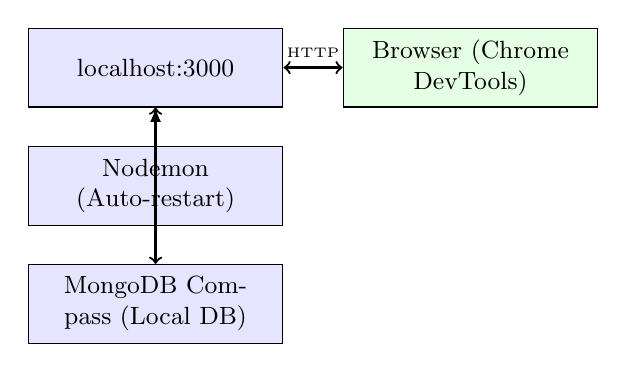
\begin{tikzpicture}[
    box/.style={rectangle, draw, fill=blue!10, text width=3cm, text centered, minimum height=1cm, font=\small},
    arrow/.style={-latex, thick}
]
    \node [box] (localhost) {localhost:3000};
    \node [box, below of=localhost, yshift=-0.5cm] (nodemon) {Nodemon (Auto-restart)};
    \node [box, below of=nodemon, yshift=-0.5cm] (mongodb_local) {MongoDB Compass (Local DB)};
    \node [box, right of=localhost, xshift=3cm, fill=green!10] (browser) {Browser (Chrome DevTools)};
    
    \draw [arrow, <->] (browser) -- node[above, font=\tiny] {HTTP} (localhost);
    \draw [arrow] (nodemon) -- (localhost);
    \draw [arrow, <->] (localhost) -- (mongodb_local);
\end{tikzpicture}
\caption{Local Development Topology}
\label{fig:dev_deployment}
\end{figure}

\subsection{Production Environment (Render.com)}

\begin{figure}[H]
\centering
\begin{tikzpicture}[
    box/.style={rectangle, draw, fill=blue!10, text width=3.5cm, text centered, minimum height=0.9cm, font=\small},
    cloud/.style={ellipse, draw, fill=orange!10, text width=3cm, text centered, minimum height=1.2cm, font=\small},
    arrow/.style={-latex, thick}
]
    \node [box, fill=yellow!10] (users) {End Users (Browsers)};
    \node [cloud, below of=users, yshift=-1cm] (render) {Render.com (Free Tier) \\Node.js Container};
    \node [cloud, below of=render, yshift=-1cm] (atlas) {MongoDB Atlas (Free Tier 512MB)};
    \node [cloud, right of=render, xshift=3.5cm] (gemini) {Google Gemini API};
    \node [cloud, left of=render, xshift=-3.5cm] (oauth) {Google OAuth};
    
    \draw [arrow, <->] (users) -- node[right, font=\tiny] {HTTPS} (render);
    \draw [arrow, <->] (render) -- (atlas);
    \draw [arrow, <->] (render) -- node[above, font=\tiny] {API} (gemini);
    \draw [arrow, <->] (render) -- node[above, font=\tiny] {OAuth} (oauth);
\end{tikzpicture}
\caption{Production Deployment on Render + MongoDB Atlas}
\label{fig:prod_deployment}
\end{figure}

\textbf{Infrastructure Specifications:}
\begin{itemize}
    \item **Compute:** Render.com Free Tier (0.1 CPU, 512MB RAM, automatic sleep after 15 min inactivity)
    \item **Database:** MongoDB Atlas M0 Free Cluster (Shared CPU, 512MB storage, 100 max connections)
    \item **CDN:** None (static files served from Node.js process)
    \item **HTTPS:** Automatic TLS certificate provisioning by Render.com
\end{itemize}

\textbf{Limitations and Trade-Offs:}
\begin{itemize}
    \item **Cold Start Latency:** First request after inactivity takes 30-60 seconds (container spin-up)
    \item **No Horizontal Scaling:** Single instance, no load balancer
    \item **Database Connection Pool:** Limited to 10 concurrent connections (free tier constraint)
\end{itemize}

\section{Summary}

This chapter presented a comprehensive architectural blueprint:

\begin{itemize}
    \item **Logical Architecture:** Client-server model with modular monolith backend
    \item **Data Architecture:** MongoDB schema design with ERD, normalization trade-offs analyzed
    \item **API Architecture:** RESTful endpoints catalog with complete request/response schemas
    \item **Component Design:** Middleware pipeline, authentication/authorization mechanisms
    \item **Security Architecture:** JWT flows, OAuth 2.0 integration, RBAC enforcement
    \item **Deployment Architecture:** Development vs. production topologies
\end{itemize}

All design decisions are grounded in actual implementation (code references provided) and justified against alternatives. The next chapter will demonstrate the translation of this design into working code, accompanied by rigorous testing and evaluation.

% End of Chapter 4
